
















































































\section{Boosting Vision-Language Generalization by Synthesizing Multi-Hop Data}
\label{sec: method}

The analysis in \cref{sec: unreliable visual perception in long-chain reasoning} shows that long-CoT reasoning does not fail for a single reason: models may make perception, reasoning, knowledge, hallucination, and other errors, and these errors often propagate once an incorrect intermediate step is carried forward through the rest of the chain.
This motivates training data beyond simply relying on, or expanding, existing vision-language RLVR training data. Specifically, the desired training data should structurally force the model to seek visual evidence at each step of long-CoT reasoning, thereby strengthening step-by-step vision-language reasoning and improving generalization across diverse scenarios.
Accordingly, we synthesize multi-hop vision-language reasoning data whose hops are designed to instantiate exactly this requirement, while ensuring that each query terminates in a specific, unambiguous numerical answer compatible with RLVR, as illustrated in \cref{fig:multihop-query-examples}.

\subsection{Multi-Hop Vision-Language Reasoning Definition}
\label{subsec:mh-vl-definition}

We first define the structure of the target multi-hop queries. To do so, we use three reasoning levels: Levels~1 and~2 describe what an individual reasoning step asks the model to do, while Level~3 describes a query that chains multiple Level~1 and Level~2 steps together.
\textbf{Level~1} is single-object perception, such as reading text or identifying object attributes, including color, shape, size, position, and category.
\textbf{Level~2} is multi-object perception, such as spatial, comparative, or counting relations across objects.
\textbf{Level~3} is multi-hop reasoning, where multiple Level~1 and Level~2 steps are chained into one query.

Within such a Level~3 query, consecutive hops can be linked in two complementary dimensions.
\textbf{Perception-level hop:} the next step changes the kind of perception being performed, for example from a Level~1 single-object judgment to a Level~2 relational judgment, or vice versa, while remaining grounded in the instances, sets, or conditions established by earlier hops.
\textbf{Instance-chain hop:} the next step moves to a new instance along an explicit dependency chain (e.g., instance A $\rightarrow$ B $\rightarrow$ C), where the next instance can only be identified from the instances, sets, or conditions established by earlier hops.

Each query must satisfy three structural conditions: (\romannumeral1) it must be Level~3, (\romannumeral2) it must combine both hop types, and (\romannumeral3) its hops must form a logically dependent chain in which earlier hops establish the instances, sets, or conditions needed for later hops.
We further prefer instance dependency chains and perception-level transitions to be intertwined as tightly as possible.
In addition, because the synthesized data is intended for RLVR, each query must terminate in a specific, unambiguous numerical answer.
This makes the final answer easy to verify for RLVR, while the logical dependence among hops means that obtaining the correct final number usually also requires the intermediate reasoning chain to be correct.
This definition is intended to rule out pseudo-multi-hop queries in which substeps are loosely connected or can be bypassed with shallow shortcuts.
Intuitively, it targets exactly the kind of failures shown in \cref{fig:qualitative_examples}: the model must repeatedly identify the correct visual evidence, then use that evidence to determine the next object, relation, or computation.

\begin{figure}[!h]
    \centering
    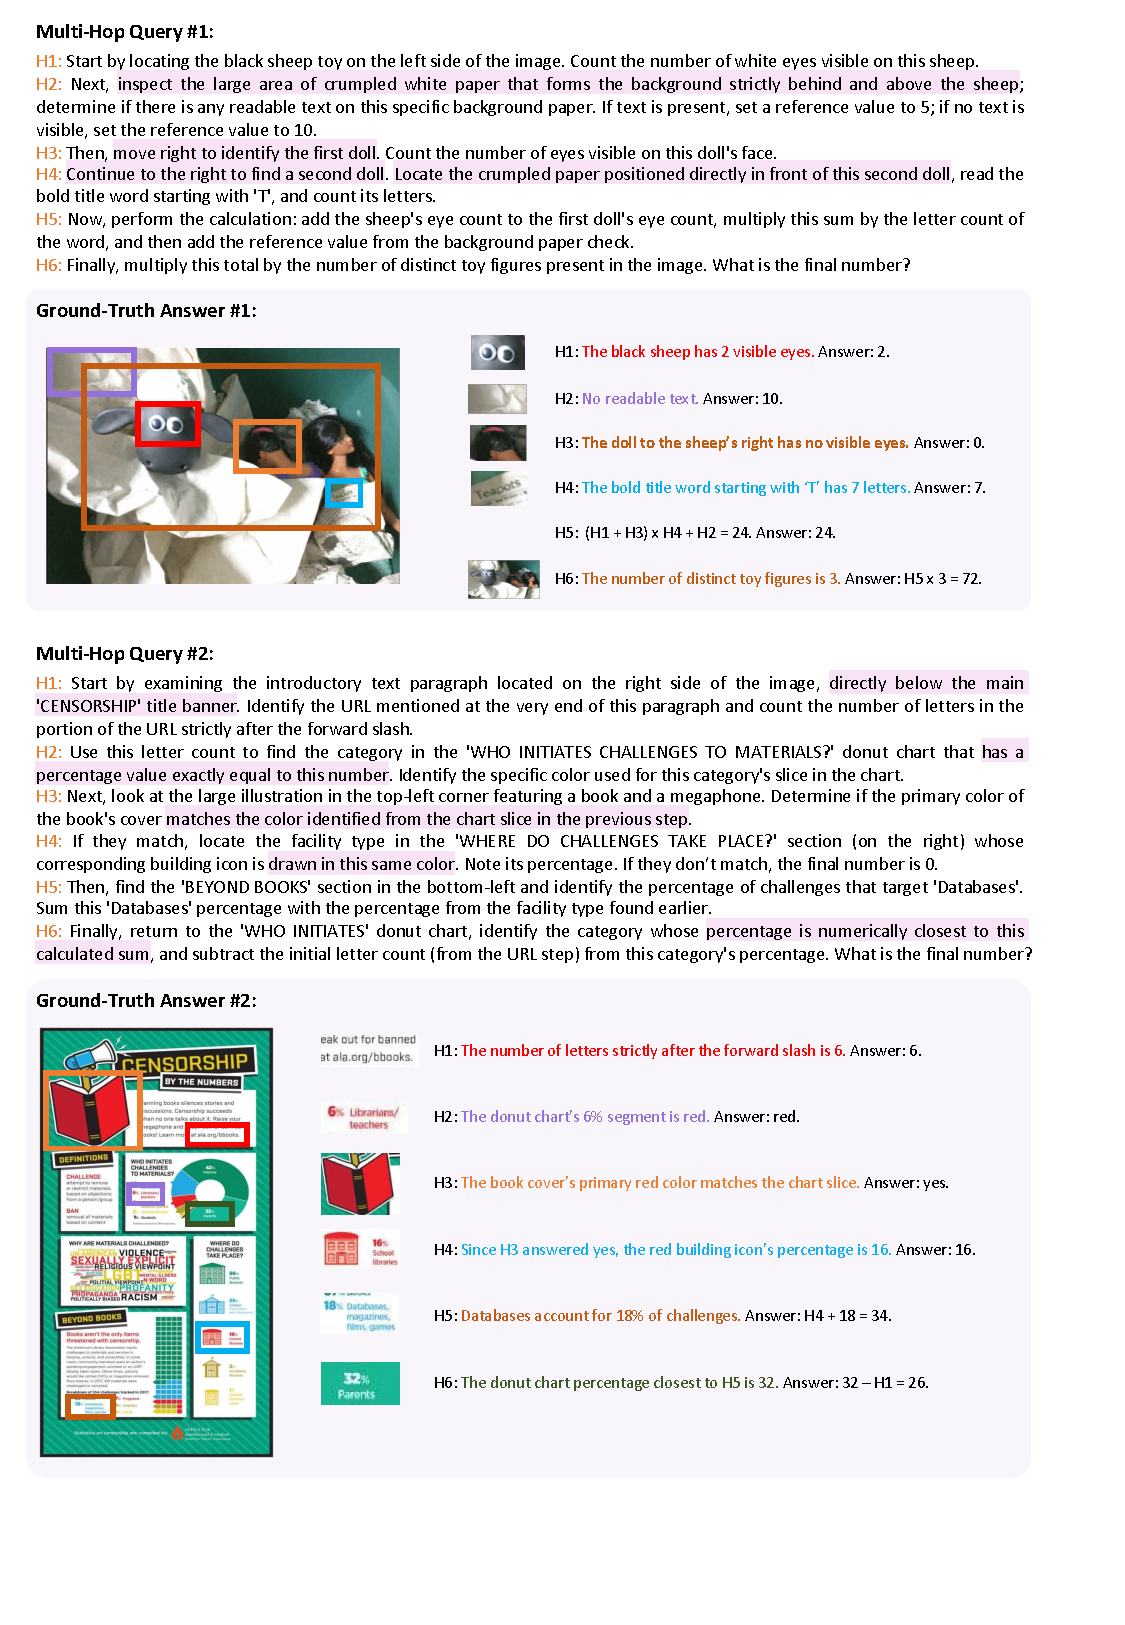
\includegraphics[width=0.97\textwidth]{imgs/multihop_examples_revised.pdf}
    \caption{Examples of synthesized multi-hop data. In each query, purple-highlighted text denotes the instance chain, meaning that the instance required at the current hop can only be identified from instances established in earlier hops. In the corresponding image, we mark the instance regions involved in each hop with colored rectangles, and the rectangle colors are aligned with the text colors of the corresponding hop-wise ground-truth answers.}
    \label{fig:multihop-query-examples}
    \vspace{-15pt}
\end{figure}

\subsection{Data Synthesis Pipeline}
\label{subsec:data-synthesis-pipeline}

Given the query definition in Section~\ref{subsec:mh-vl-definition}, we next describe how candidate multi-hop queries are synthesized. We build the dataset through a three-stage synthesis pipeline that operationalizes this design goal into trainable RLVR data (see \cref{fig:example_image}(a) for the full four-stage workflow, where this subsection covers Stages~1--3 and \cref{subsec:ground-truth-annotation} covers Stage~4).
The pipeline is designed so that the final queries are not only complex, but also structurally aligned with the long-CoT setting we care about: multiple intermediate hops, each grounded in visual evidence and required for later hops.

\textbf{Stage 1: Category Identification.}
We first identify the candidate visual entities that later hops can operate over.
Given an input image, we use a VLM (Qwen3-VL-235B-A22B-Thinking) to identify semantic categories present in the image, yielding a list of semantic categories (e.g., ``car,'' ``person,'' ``sign'') without localization.

\textbf{Stage 2: Instance Segmentation.}
We then resolve these categories into concrete instances, because hop-based reasoning must be anchored to particular objects rather than generic labels.
For each identified semantic category, we use SAM3 to generate segmentation masks and bounding boxes for candidate instances of that category where possible, producing a set of individual instances with spatial localization.

\textbf{Stage 3: Multi-Hop Query Generation.}
This stage is where we convert detected instances into training questions that enforce chained visual reasoning rather than isolated recognition.
We form combinations of 3--6 instances and use Qwen3-VL-235B-A22B-Thinking to generate multi-hop queries for each combination.
The model receives the original image plus cropped patches of each instance, where the patches are used only at design time to help identify the appearance and location of each instance. The full prompt used for multi-hop query synthesis is provided in Appendix~\ref{app:multihop-prompt}.
Crucially, to address the failure modes identified in \cref{sec: unreliable visual perception in long-chain reasoning}, we impose several constraints on each synthesized query: it must (i) involve as many instances as possible from the selected combination while remaining answerable from the original image alone; (ii) describe objects only by spatial, contextual, or visual attributes; (iii) terminate in a specific, unambiguous numerical answer; and (iv) avoid any reference to segmentation masks, bounding boxes, or patch images.
These constraints prevent the synthesis process from leaking shortcuts that would let the model solve the query from auxiliary cues unavailable at training or test time.
In addition, reasoning hops must form a logically dependent chain: each hop must either change the perception level or move along an instance dependency chain, while earlier hops establish the instances, sets, or conditions needed for later hops.
As a result, the synthesized queries better mirror the structure of long-CoT reasoning: the model must recover and retain intermediate visual evidence and use it to determine the next step, rather than rely on an early guess or a language-only heuristic.


\subsection{Ground-Truth Annotation and Difficulty Calibration}
\label{subsec:ground-truth-annotation}

After the synthesis pipeline in Section~\ref{subsec:data-synthesis-pipeline} produces candidate queries, we introduce a separate Stage~4 with two complementary components: \emph{ground-truth annotation} and \emph{difficulty calibration}.
In this stage, ground-truth annotation filters out low-quality queries and provides reliable numerical ground-truth answers for the retained ones, while difficulty calibration uses these verified answers to remove queries that are too easy.

\textbf{Stage 4: Ground-Truth Annotation and Difficulty Calibration.}
For each generated query, four annotators from our data annotation team independently solve it.
During ground-truth annotation, we discard queries where annotators report ambiguous references or other quality issues, and for queries that pass, we take the shared final numerical answer (all four must agree) as the ground truth.
For difficulty calibration, we evaluate the retained queries on a weaker model with eight sampled responses per query, using the verified ground-truth answers as reference; queries on which the weaker model achieves $100\%$ accuracy are removed as too easy, and the remaining queries form our final dataset with verified difficulty and reliable ground-truth annotations.

Together, the pipeline functions as a scalable data synthesis workflow: from raw images to verified multi-hop queries, it can be applied to broad image collections with sufficient detectable instances, while maintaining quality control through human and model-based verification.
In this way, the synthesized data is not merely harder data.
It is constructed to expose the model to the same kind of chained evidence use that long-CoT reasoning requires in practice, thereby providing a more suitable training signal for improving robustness and generalization across diverse visual scenarios.
A direct comparison between the typical vision-language reasoning question in \cref{fig:qualitative_examples} and the synthesized multi-hop data in \cref{fig:multihop-query-examples} makes this difference concrete: simply scaling existing RLVR-style data often still leaves shallow or loosely coupled solution paths, whereas our synthesized data enforces hop-wise dependency and repeated visual re-grounding throughout the chain.
This structural gap is precisely why relying on, or merely expanding, existing vision-language RLVR training data is insufficient.
